%% Le lingue utilizzate, che verranno passate come opzioni al pacchetto babel. Come sempre, l'ultima indicata sarà quella primaria.
%% Se si utilizzano una o più lingue diverse da "italian" o "english", leggere le istruzioni in fondo.
\def\thudbabelopt{english,italian}
%% Valori ammessi per target: bach (tesi triennale), mst (tesi magistrale), phd (tesi di dottorato).
%% Valori ammessi per aauheader: '' (vuoto -> nessun header Alpen Adria Univeristat), aics (Department of Artificial Intelligence and Cybersecurity), informatics (Department of Informatics Systems). Il nome del dipartimento è allineato con la versione inglese del logo UniUD.
%% Valori ammessi per style: '' (vuoto -> stile moderno), old (stile tradizionale).
\documentclass[target=bach,aauheader=,style=]{thud}

%% --- Informazioni sulla tesi ---
%% Per tutti i tipi di tesi
% Scommentare quello di interesse, o mettete quello che vi pare
\course{Informatica}
%\course{Internet of Things, Big Data e Web}
%\course{Matematica}
%\course{Comunicazione Multimediale e Tecnologie dell'Informazione}
\title{Comparazione sperimentale \\ di algoritmi di cifratura lightweight \\ su microcontrollori embedded}
\author{Jacopo Plozner}
\supervisor{Prof.\ Marino Miculan}
%\cosupervisor{Arch.\ Rambaldo Melandri \and Dott.\ Giorgio Perozzi}
\tutor{Dott.\ Paolo Casoto}
%% Campi obbligatori: \title, \author e \course.
%% Altri campi disponibili: \reviewer, \tutor, \chair, \date (anno accademico, calcolato in automatico), \rights
%% Con \supervisor, \cosupervisor, \reviewer e \tutor si possono indicare più nomi separati da \and.
%% Per le sole tesi di dottorato:
%\phdnumber{313}
%\cycle{XXVIII}
%\contacts{Via della Sintassi Astratta, 0/1\\65536 Gigatera --- Italia\\+39 0123 456789\\\texttt{http://www.example.com}\\\texttt{inbox@example.com}}

%% --- Pacchetti consigliati ---
%% pdfx: per generare il PDF/A per l'archiviazione. Necessario solo per la versione finale
\usepackage[a-1b]{pdfx}
%% hyperref: Regola le impostazioni della creazione del PDF... più tante altre cose. Ricordarsi di usare l'opzione pdfa.
\usepackage[pdfa]{hyperref}
%% tocbibind: Inserisce nell'indice anche la lista delle figure, la bibliografia, ecc.

%% --- Stili di pagina disponibili (comando \pagestyle) ---
%% sfbig (predefinito): Apertura delle parti e dei capitoli col numero grande; titoli delle parti e dei capitoli e intestazioni di pagina in sans serif.
%% big: Come "sfbig", solo serif.
%% plain: Apertura delle parti e dei capitoli tradizionali di LaTeX; intestazioni di pagina come "big".
\usepackage{float} % figure EXACTLY here
\usepackage{MnSymbol} % simboli

\begin{document}
\maketitle

%% Dedica (opzionale)
\begin{dedication}
	Al mio cane,\par per avermi ascoltato mentre ripassavo le lezioni.
\end{dedication}

%% Ringraziamenti (opzionali)
\acknowledgements


%% Sommario (opzionale)
\abstract


%% Indice
\tableofcontents

%% Lista delle tabelle (se presenti)
%\listoftables

%% Lista delle figure (se presenti)
%\listoffigures

%% Corpo principale del documento
\mainmatter

%% Parte
%% La suddivisione in parti è opzionale; solitamente sono sufficienti i capitoli.
%\part{Parte}

%% Capitolo
\chapter{Introduzione}

    %% Sezione
    \section{Titolo della Sezione}


    %% Sottosezione
    \subsection{Sottosezione}

\chapter{Background}

    \section{Crittografia}
    La crittografia è la scienza, da alcuni definita anche \textit{arte}, che si occupa dello studio e della creazione di tecniche matematiche per la sicurezza di sistemi informatici e comunicazioni digitali.\cite{moderncrypto}\\
    Tra le molte tecniche troviamo i cifrari (cipher), algoritmi parametrizzati da una chiave (key) che trasformano un testo in chiaro (plaintext) in un testo cifrato (ciphertext).\\
    Le operazioni di cifratura \textit{E} (encryption) e decifratura \textit{D} (decryption) tramite la chiave \textit{K} e il rapporto tra plaintext \textit{P} e ciphertext \textit{C} possono essere rappresentati con le funzioni:
    \[E_K(P)=C \qquad , \qquad D_K(C)=P\]
    Un principio fondamentale della crittografia, che pone le basi per una progettazione sicura di un cifrario, è quello di Kerckhoffs:
    \begin{quote}
        La sicurezza di un sistema non deve dipendere dalla segretezza dell'algoritmo di cifratura usato, ma da quella della chiave.
    \end{quote}
    Claude Shannonn lo riformula con "Il nemico conosce il sistema" (\textit{Communication Theory of Secrecy Systems}); un cifrario quindi è considerato sicuro solo se garantisce la sua robustezza anche, e soprattutto, nel caso in cui un eventuale malintenzionato ne conosca tutti i dettagli implementativi.\\
    Questo consente ai crittografi di rendere pubbliche le loro scelte progettuali, in modo che il loro lavoro possa essere studiato e analizzato da altri esperti.
    
    Gli algoritmi di cifratura classici si dividono in due categorie: a chiave simmetrica e a chiave asimmetrica.

        \subsection{Crittografia simmetrica}
        Conosciuta anche come \textit{crittografia a chiave privata}, in questo scenario, due parti condividono una chiave segreta, che utilizzano per comunicare in modo cifrato.\\
        Le operazioni di cifratura e decifratura dei messaggi avvengono con la stessa chiave, da qui la definizione di \textit{simmetrica}. \\
        Una prima grande distinzione tra gli algoritmi in questa categoria si può fare sulla base di come operano sul messaggio: cifrari a blocco (\textit{Block ciphers}) e cifrari a flusso (\textit{Stream ciphers}).

            \subsubsection{Cifrari a blocco}
            Un cifrario a blocco è un algoritmo che opera su una quantità fissata di bit, detta appunto \textit{blocco}. \\
            Può essere descritto come una permutazione parametrizzata da una chiave\cite{moderncrypto}:
            \[F:\{0,1\}^b \times \{0,1\}^k \rightarrow \{0,1\}^b\]
            dove \textit{b} è la lunghezza del blocco e \textit{k} la lunghezza della chiave. 

            Diverse sono le architetture di cifrari a blocco presenti in letteratura, ma la maggior parte condivide le stesse idee base, teorizzate da Claude Shannon (\textit{A Mathematical Theory of Cryptography}, 1945):
            \begin{itemize}
                \item \textbf{Confusion}: il rapporto tra plaintext, ciphertext e chiave deve essere reso il piú complesso possibile. Questa proprietà viene raggiunta con l'utilizzo di tecniche di \textbf{sostituzione}, applicate all'intero messaggio diviso in gruppi di pochi bit, implementate tramite Look Up Table (S-Boxes)
                \item \textbf{Diffusion}: ogni cambiamento, anche il più piccolo, deve avere effetto su almeno metà blocco. Proprietá ottenuta tramite \textbf{permutazione} dei bit, grazie a semplici circuiti dedicati oppure una complicata implementazione software.
            \end{itemize}

            Architetture comuni:
            \begin{description}
                \item[Substitution-Permutation Networks (SPN)] Implementazione diretta del paradigma Confusion\&Diffusion\cite{moderncrypto}, sono infatti cifrari composti da divesi round di sostituzioni e permutazioni\cite{handcypto}.

                Prima dei round c'è la fase detta \textbf{Key Schedule}, in cui la chiave principale (\textit{master key}) viene usata per generare le sotto-chiavi utilizzate in ciascun round (\textit{round keys}).\\
                Ogni round è composto solitamente dalle seguenti fasi\cite{moderncrypto}:                
                \begin{enumerate}
                    \item Round key mixing: la round key corrispondente viene sommata al messaggio. \[M = M \oplus RK_i\]
                    \item Substitution: sostituzione dei byte del messaggio $(M:m_0||\ ...\ ||m_n)$ sulla base delle S-Box. \[M=S(m_0)||\ ...\ ||S(m_n)\]
                    \item Permutation: permutazione dei bit di M.
                \end{enumerate}
                L'output di ciascun round è l'input del successivo.\\
                Dopo l'ultimo round il messaggio è sommato all'ultima sotto-chiave.
                \begin{figure}[h]
                    \centering
                    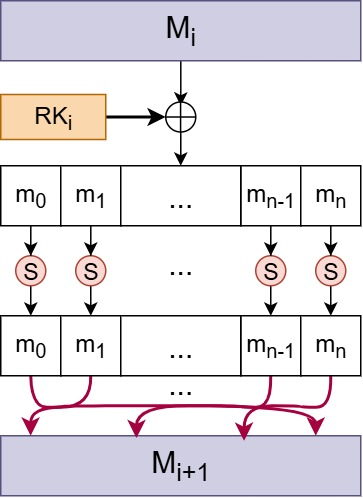
\includegraphics[width=0.5\linewidth]{img/spn_round.jpg}
                    \caption{SPN round}
                    \label{fig:placeholder}
                \end{figure}
                \item[Feistel Networks \cite{moderncrypto}] Approccio teorizzato da Horst Feistel (\textit{Cryptography and Computer Privacy}, 1973), al contrario degli SPN, presenta il vantaggio di poter utilizzare come componente base una funzione non invertibile \textit{RF} (\textit{round function}).\\
                Anche in questo caso, operando a round, è presente una fase inziale di \textit{key schedule} per espandere la \textit{master key K} nelle relative \textit{round keys $RK_i$}.\\
                Questi cifrari operano iterativamente sul messaggio, considerandolo come due parti di lunghezza uguale ($M_i:L_i||R_i$), nel seguente modo:
                \begin{enumerate}
                    \item $L_{i+1} = R_i$
                    \item $R_{i+1} = L_i \oplus RF_{RK_i}(R_i)$
                \end{enumerate}
                \begin{figure}[h]
                    \centering
                    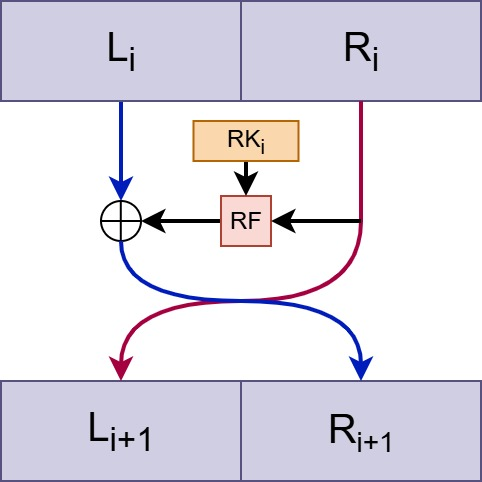
\includegraphics[width=0.5\linewidth]{img/feistel_round.jpg}
                    \caption{Feistel Network round}
                    \label{fig:placeholder}
                \end{figure}
                \item[Add-Rotate-XOR (ARX)\cite{sparx}] Classe di cifrari progettati utilizando soltanto semplici operazioni di \textit{addizione modulare} ($\boxplus$), \textit{rotazione} ($\lll, \ggg$) e \textit{XOR} ($\oplus$).
            \end{description}
            
            Di per sé non è una soluzione sicura, soprattutto in presenza di più blocchi da cifrare, in quanto presenta un comportamento deterministico: applica, a parità di chiave, sempre la stessa permutazione. Occorre adottare delle particolari tecniche, chiamate \textit{Modes of Operation}, che utilizzano il cifrario a blocco come primitiva e non come unica risorsa. \cite{handcypto, computernet}
            % modes
            
            \subsubsection{Cifrari a flusso}
            Un cifrario a flusso è un algoritmo che cifra un messaggio combinandolo con un flusso pseudocasuale di simboli (\textit{keystream}). Ogni simbolo del plaintext è cifrato con il simbolo corrispondente del keystream.\\
            La componente base di un cifrario a flusso è solitamente un \textit{LFSR} (\textit{linear-feedback shift register}), uno strumento utilizzato per la generazione pseudocasuale di numeri, con buone proprietà statistiche. Un LFSR consiste in un array di registri da un bit ciascuno, i cui valori ne rappresentano lo stato. Lo stato è aggiornato ad ogni intervallo dato, shiftando i valori dei registri verso destra, mentre il nuovo valore del primo registro da sinistra è calcolato tramite lo XOR di un sottoinsieme dei valori attuali. In un dato momento, il valore dell'ultimo registro a destra rappresenta l'output del LFSR.\cite{moderncrypto}
            \begin{figure}[h]
                \centering
                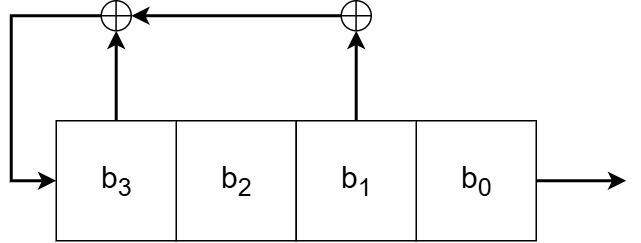
\includegraphics[width=0.5\linewidth]{img/lfsr.jpg}
                \caption{LFSR}
                \label{fig:placeholder}
            \end{figure}
        \subsection{Crittografia asimmetrica}

    \section{Sistemi embedded}
    
        
    
\chapter{Algoritmi}

\chapter{Test e valutazione}

\chapter{Conclusione}



%% Fine dei capitoli normali, inizio dei capitoli-appendice (opzionali)
\appendix

%\part{Appendici}

\chapter{Appendice}


%% Parte conclusiva del documento; tipicamente per riassunto, bibliografia e/o indice analitico.
\backmatter

%% Riassunto (opzionale)
%\summary

%% Bibliografia (praticamente obbligatoria)
\bibliographystyle{plain_\languagename}%% Carica l'omonimo file .bst, dove \languagename è la lingua attiva.
%% Nel caso in cui si usi un file .bib (consigliato)
\bibliography{thud}

%% Nel caso di bibliografia manuale, usare l'environment thebibliography.

%% Per l'indice analitico, usare il pacchetto makeidx (o analogo).

\end{document}